\documentclass[11pt,a4paper,oneside]{report}

\usepackage[utf8]{inputenc}
\usepackage[T1]{fontenc}
\usepackage[english]{babel}
\usepackage{lmodern}
\usepackage{microtype}
\usepackage{csquotes}

\usepackage[a4paper,margin=2.5cm]{geometry}
\usepackage{setspace}
\onehalfspacing

\usepackage{booktabs}
\usepackage{array}
\usepackage{graphicx}
\usepackage{caption}
\usepackage{subcaption}
\usepackage{siunitx}
\sisetup{group-separator={,}, detect-all}
\usepackage{listings}
\usepackage{xcolor}
\lstset{
basicstyle=\ttfamily\small, columns=fullflexible, keepspaces=true, breaklines=true,
frame=single, keywordstyle=\color{blue!60!black}, commentstyle=\color{gray},
showstringspaces=false, language=Python }

\usepackage{amsmath,amssymb}

\usepackage[backend=biber,style=ieee,sorting=nyt]{biblatex}
\addbibresource{references.bib}

\usepackage[hidelinks]{hyperref}
\usepackage{cleveref}

\newcommand{\code}[1]{\texttt{#1}}
\newcommand{\pkg}{\code{llm-semantic-chunker}}
\newcommand{\hitk}[1]{Hit@#1}
\newcolumntype{L}[1]{>{\raggedright\arraybackslash}p{#1}}

\begin{document}

\begin{titlepage}
  \centering
  \vspace*{3cm}
  {\LARGE\bfseries LLM-Based Semantic Chunking\\for Retrieval-Augmented Generation\par}
  \vspace{0.6cm}
  {\large A Comparison with Rule-Based Chunking Strategies\par}
  \vspace{2.5cm}
  {\large Bachelor's Thesis\par}
  \vspace{0.4cm}
  {\large Ivan Antunovic\par}
  \vspace{2cm}
  {\large Supervisor: Dr.\ Marian Lux\par}
  \vspace{0.4cm}
  {\large University of Vienna\par}
  \vfill
  {\large September 30, 2026\par}
\end{titlepage}

\chapter*{Abstract}
The use of large language models (LLMs) is more widespread than ever, and with their
integration into more and more industries a further rise seems inevitable. However, these
models are trained on past data and generate responses based on probabilities, which can
lead to hallucinations. Retrieval-augmented generation (RAG) counteracts this problem by
supplying the model with relevant documents. To do so, a RAG system has to split the
documents into chunks, a pre-processing step that determines what can be retrieved and
thereby the accuracy of the answers. In this thesis, an LLM-based chunker is implemented as
an alternative to rule-based chunking strategies and published as a Python library on
PyPI. It uses a small local model that reads the document sentence by sentence and decides
where the topic changes; optional post-processing steps are meant to improve retrieval
further. The chunker is evaluated on three documents of different structure (a technical
standard, a PDF handbook and narrative prose) against five baselines tuned to the same mean
chunk length: four splitters from LangChain and the same chunker without the model. The
statistical analysis uses paired McNemar tests with a Holm correction over 30 comparisons,
with 400 to 549 questions per document. In six of the 30 comparisons, the LLM chunker
retrieves significantly more answers than the splitters that cut sentences apart, but it is
not significantly better than the splitters that keep sentences intact or than the same
chunker without the model. This indicates that its advantage comes from respecting sentence
boundaries rather than from the model's topic decisions. Heading detection and topic labels
did not improve retrieval significantly, and the filter for chunks without substantive
content even lowered it. In practice, a length-matched recursive splitter that prefers
sentence ends reaches comparable hit rates in a few seconds, against a mean of about three
hours per document on an \SI{8}{\giga\byte} MacBook Air.

\tableofcontents

\chapter{Introduction}
\label{ch:intro}

\section{Motivation}

Large language models (LLMs) demonstrate high accuracy by storing factual knowledge in
their parameters, yet they remain prone to hallucinations, and their ability to access and
update knowledge is limited~\cite{lewis2020rag}. Retrieval-augmented generation (RAG)
addresses these shortcomings by combining the parametric language generator of an LLM with
a non-parametric external document index, from which relevant information is retrieved to
generate more accurate answers~\cite{lewis2020rag}. Within the RAG pipeline, document
chunking is the pre-processing step that splits the text into units and thereby defines the
search granularity of the vector index~\cite{smigielski2026chunking}.

Many chunking variants exist for this step, but they differ in accuracy and are not
suitable for every document type or domain. Recent research introduced a newer mechanism,
LLM-based chunking, which dynamically identifies narrative topic shifts to improve the
quality of each vector embedding~\cite{duarte2024lumberchunker}. However, LLM-driven
segmentation introduces a considerable computational latency compared to the existing
baselines, as the experiments with LumberChunker showed~\cite{duarte2024lumberchunker}.

Furthermore, empirical evidence suggests that on real-world documents, sentence-level
positional proximity already provides a strong natural heuristic for semantic shifts, so
that the computational overhead is not justified by the gain~\cite{qu-etal-2025-semantic}.
This motivates an evaluation of whether LLM-based chunking brings a real advantage over
length-matched baselines, or whether preserving the integrity of sentences is already
sufficient for effective retrieval.

\section{Problem statement and research question}
\label{sec:problem}

The research question is: \emph{Does a local language model place better chunk boundaries
than rule-based chunking techniques, and under which conditions?} Secondary questions
concern the effect of the optional features of the library: heading detection, the
low-information filter, topic enrichment and the choice of the split point when a chunk
exceeds the size cap.

\chapter{Background and Related Work}
\label{ch:background}

\section{Chunking in retrieval-augmented generation}
\label{sec:rag_chunking}

Standard large language models (LLMs) struggle with knowledge-intensive tasks because their
internal knowledge is limited by a static training cut-off and their output lacks
verifiable sources~\cite{lewis2020rag}. Retrieval-augmented generation (RAG) resolves these
limitations by coupling pre-trained parametric generators (such as BART) with
non-parametric memory in the form of an external dense vector index~\cite{lewis2020rag}. In
a RAG pipeline, raw source documents are first split into retrievable text units, the
so-called \emph{chunks}~\cite{smigielski2026chunking}, which are then converted into dense
vector representations by a neural encoder and finally searched through maximum inner
product search (MIPS) or approximate nearest-neighbour algorithms~\cite{lewis2020rag}.

This segmentation is a pre-processing step that determines the quality of the subsequent
vector index~\cite{smigielski2026chunking}. Downstream components, such as cross-encoder
rerankers, have to rely on the initial segmentation; errors made during this step cannot be
repaired later, and the subsequent components are forced to process chunks that are either
truncated or contextually degraded~\cite{duarte2024lumberchunker}.

Chunking can fail in two ways. Chunks that are too small or cut mid-sentence lack
sufficient factual context, which leads to retrieval failures and a higher risk of
hallucinations by the LLM. Conversely, chunks that are too large contain irrelevant
content, which dilutes the vector embedding and creates a semantic misalignment with the
query vector during dense retrieval~\cite{smigielski2026chunking}.

Despite its decisive role in a RAG pipeline, chunking has historically been treated as an
arbitrary pre-processing step done through fixed character cuts rather than as an
architectural variable~\cite{qu-etal-2025-semantic}. For comparative studies, recent
literature emphasises the need to isolate chunking from the rest of the RAG pipeline in
order to guarantee consistency across the compared splitting
variants~\cite{smigielski2026chunking}.

\section{Rule-based and embedding-based strategies}
\label{sec:rule_based}

\begin{figure}[htbp]
  \centering
  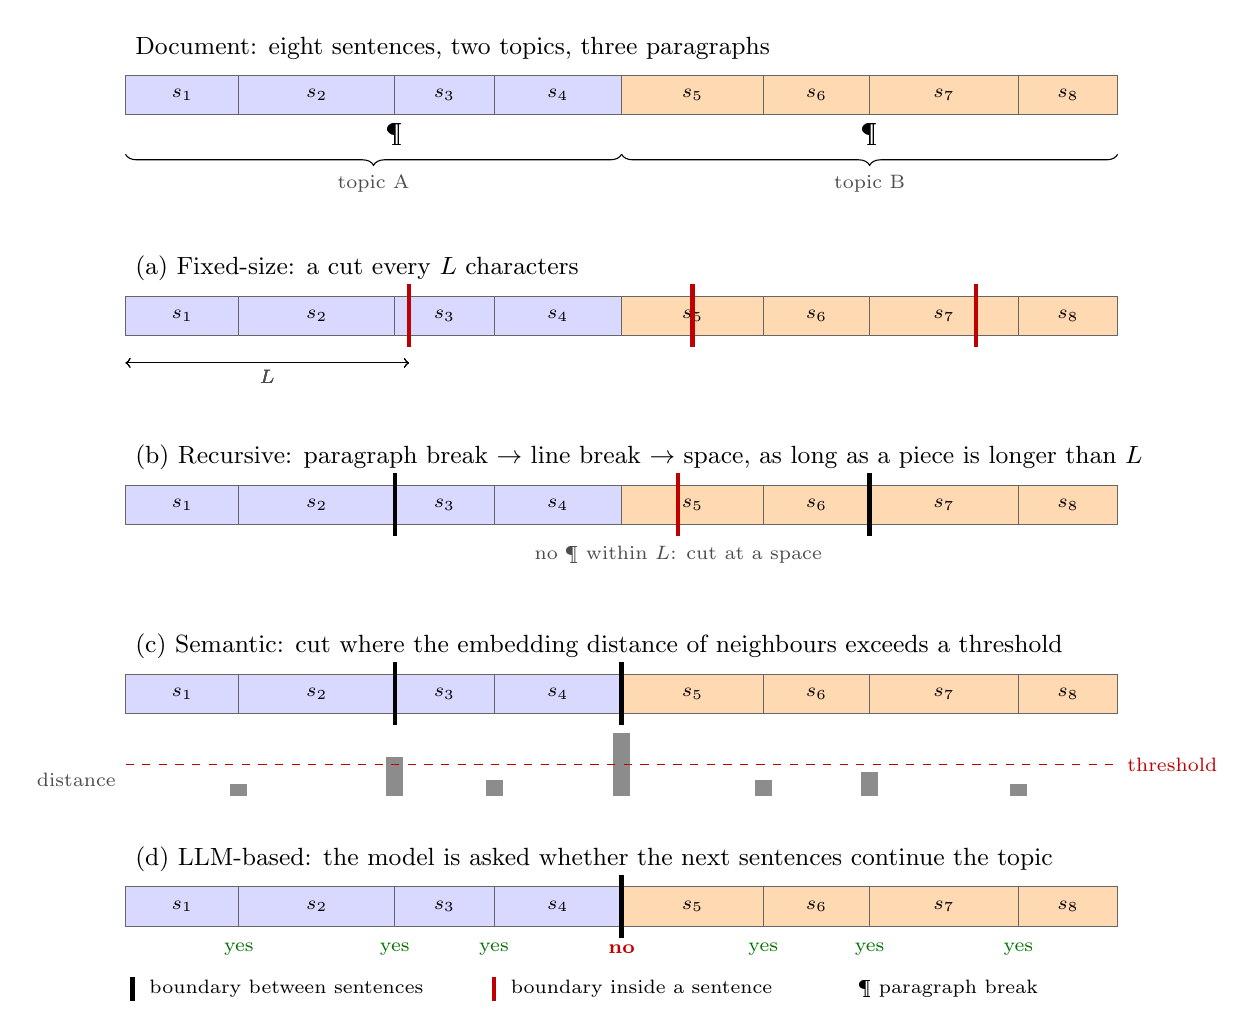
\begin{tikzpicture}[x=0.9cm,y=1cm,
      sent/.style={draw=black!60, line width=0.3pt},
      cut/.style={line width=1.6pt, black},
      badcut/.style={line width=1.6pt, red!75!black},
      lbl/.style={anchor=west, font=\small},
      note/.style={font=\scriptsize, text=black!70}]
    \colorlet{topicA}{blue!15}
    \colorlet{topicB}{orange!30}
    % one row of eight sentences; #1 = y position of the row
    \newcommand{\sentstrip}[1]{%
      \foreach \a/\b/\t/\n in {0/1.6/A/1, 1.6/3.8/A/2, 3.8/5.2/A/3, 5.2/7.0/A/4,
                               7.0/9.0/B/5, 9.0/10.5/B/6, 10.5/12.6/B/7, 12.6/14.0/B/8}{%
        \draw[sent, fill=topic\t] (\a,#1) rectangle (\b,#1+0.5);
        \node[font=\scriptsize] at ({(\a+\b)/2},#1+0.25) {$s_{\n}$};}}
    \newcommand{\cutat}[3][cut]{\draw[#1] (#2,#3-0.15) -- (#2,#3+0.65);}

    % document
    \node[lbl] at (0,11.35) {Document: eight sentences, two topics, three paragraphs};
    \sentstrip{10.5}
    \foreach \x in {3.8,10.5} \node[font=\small] at (\x,10.25) {\P};
    \draw[decorate, decoration={brace, mirror, amplitude=4pt}] (0,10.0) -- (7.0,10.0)
      node[midway, below=4pt, note] {topic A};
    \draw[decorate, decoration={brace, mirror, amplitude=4pt}] (7.0,10.0) -- (14.0,10.0)
      node[midway, below=4pt, note] {topic B};

    % (a) fixed-size
    \node[lbl] at (0,8.55) {(a) Fixed-size: a cut every $L$ characters};
    \sentstrip{7.7}
    \foreach \x in {4.0,8.0,12.0} \cutat[badcut]{\x}{7.7}
    \draw[<->, note] (0,7.35) -- (4.0,7.35) node[midway, below=-1pt] {$L$};

    % (b) recursive
    \node[lbl] at (0,6.15) {(b) Recursive: paragraph break $\rightarrow$ line break
      $\rightarrow$ space, as long as a piece is longer than $L$};
    \sentstrip{5.3}
    \cutat{3.8}{5.3} \cutat{10.5}{5.3} \cutat[badcut]{7.8}{5.3}
    \node[note, anchor=north] at (7.8,5.15) {no \P\ within $L$: cut at a space};

    % (c) semantic
    \node[lbl] at (0,3.75) {(c) Semantic: cut where the embedding distance of neighbours
      exceeds a threshold};
    \sentstrip{2.9}
    \foreach \x/\h in {1.6/0.15, 3.8/0.5, 5.2/0.2, 7.0/0.8, 9.0/0.2, 10.5/0.3, 12.6/0.15}
      \fill[black!45] (\x-0.12,1.85) rectangle (\x+0.12,1.85+\h);
    \draw[dashed, red!75!black] (0,2.25) -- (14.0,2.25)
      node[right, note, text=red!75!black] {threshold};
    \node[note, anchor=east] at (0,2.05) {distance};
    \cutat{3.8}{2.9} \cutat{7.0}{2.9}

    % (d) LLM-based
    \node[lbl] at (0,1.05) {(d) LLM-based: the model is asked whether the next sentences
      continue the topic};
    \sentstrip{0.2}
    \foreach \x in {1.6,3.8,5.2,9.0,10.5,12.6}
      \node[note, text=green!45!black] at (\x,-0.1) {yes};
    \node[note, text=red!75!black, font=\scriptsize\bfseries] at (7.0,-0.1) {no};
    \cutat{7.0}{0.2}

    % legend
    \draw[cut] (0.1,-0.75) -- (0.1,-0.45);
    \node[lbl, font=\scriptsize] at (0.2,-0.6) {boundary between sentences};
    \draw[badcut] (5.2,-0.75) -- (5.2,-0.45);
    \node[lbl, font=\scriptsize] at (5.3,-0.6) {boundary inside a sentence};
    \node[lbl, font=\scriptsize] at (10.2,-0.6) {\P\ paragraph break};
  \end{tikzpicture}
  \caption{The chunking strategies of \cref{sec:rule_based,sec:llm_chunking}, applied to the
  same schematic document. Fixed-size splitting (a) ignores the text and cuts inside
  sentences. Recursive splitting (b) prefers paragraph breaks but falls back to spaces
  inside a long paragraph. Semantic chunking (c) cuts where consecutive sentence
  embeddings differ strongly, which can also produce boundaries within a topic ($s_2|s_3$).
  LLM-based chunking (d) asks a language model at each step and cuts only at the topic
  change.}
  \label{fig:strategies}
\end{figure}

\Cref{fig:strategies} illustrates the strategies discussed in this chapter on one schematic
document. \emph{Fixed-size chunking} (\cref{fig:strategies}a) splits a source document
into uniform segments based on a predetermined character or token
limit~\cite{qu-etal-2025-semantic}. Although the
procedure is computationally simple and deterministic, it disregards syntax and thematic
organisation~\cite{smigielski2026chunking}. This leads to chunks that are cut mid-topic and
thus to a potential degradation in retrieval quality~\cite{qu-etal-2025-semantic}. To
mitigate these effects, RAG implementations let consecutive fixed-size segments overlap in
a sliding window, typically by \SIrange{10}{20}{\percent} of the chunk
length~\cite{smigielski2026chunking}. However, a recent empirical evaluation found that
overlap provides no measurable improvement in answer quality and only increases the
indexed text and the memory overhead~\cite{bennani2026chunking}.

In contrast, \emph{recursive character splitting} (\cref{fig:strategies}b) traverses the document through an
ordered hierarchy of typographical separators and thereby preserves its structure where
possible~\cite{duarte2024lumberchunker}. Typically, such splitters cascade through
paragraph breaks, line breaks, sentence punctuation and finally spaces: when a segment
still exceeds the size limit, the algorithm moves one step down the hierarchy to find a
split point~\cite{duarte2024lumberchunker}.

Embedding-based strategies differ from these typographical heuristics in that they detect
boundaries semantically. \emph{Semantic chunking} (\cref{fig:strategies}c) converts individual sentences or passages
into dense vector embeddings, numerical representations in a high-dimensional space,
using models such as Sentence-BERT (SBERT)~\cite{reimers2019sbert}. The cosine distance
between consecutive segments then determines whether a thematic shift has occurred. More
advanced approaches such as Max--Min semantic chunking compare the similarity of each
incoming sentence to the current chunk with the minimum similarity within that chunk, so
that the text is split without a fixed window size~\cite{kiss2025maxmin,
smigielski2026chunking}. However, the benefit of semantic chunking depends strongly on the
data. On artificially stitched datasets with high topic diversity, it preserves topic
boundaries better than recursive algorithms, but on real-world documents, which already
provide natural cues for topic boundaries, the retrieval accuracy does not differ
substantially while the computational cost is higher~\cite{qu-etal-2025-semantic}. The
additional cost, latency and memory needed to compute sentence-level embeddings are
therefore rarely justified for standard structured text~\cite{qu-etal-2025-semantic}.

\section{LLM-based chunking strategies}
\label{sec:llm_chunking}

LLM-based segmentation strategies replace distance thresholds with generative models that
identify semantic shifts in a document (\cref{fig:strategies}d)~\cite{smigielski2026chunking}. Earlier work in this
field includes LumberChunker, which divides a text into paragraphs and assigns them
sequential IDs starting at 1. Consecutive paragraphs are collected into a group until a
target token count is exceeded, and the group is then submitted to an LLM with a prompt
that asks for the ID of the paragraph at which the narrative or topical focus
changes~\cite{duarte2024lumberchunker}.

On a benchmark of \num{3000} question--answer pairs from 100 narrative books of Project
Gutenberg, LumberChunker reached a Recall@20, the share of relevant passages retrieved
among the top 20 chunks, of \SI{77.92}{\percent}, outperforming the recursive chunking
baseline with \SI{74.35}{\percent}~\cite{duarte2024lumberchunker}.

However, these improvements in retrieval accuracy come with high operational and
computational costs~\cite{smigielski2026chunking}. LLM-based chunking is generally the most
expensive form of pre-processing. Because each prompt depends on the boundary returned for the previous
passage, the queries cannot be parallelised~\cite{duarte2024lumberchunker}. The processing
time therefore grows with the size of the document~\cite{duarte2024lumberchunker}.

\section{Shortcomings in current literature and methodological commitments}
\label{sec:commitments}

Existing literature on document segmentation for RAG shows substantial methodological
limitations. First, comparative evaluations frequently test chunking strategies without
calibrating the baselines to the average chunk length of the LLM
splitters~\cite{qu-etal-2025-semantic}. For example, in the evaluation of LumberChunker,
the recursive baselines averaged 399 tokens per chunk, while the LLM chunker produced a
mean of 334 tokens~\cite{duarte2024lumberchunker}. Without normalising the baseline
lengths, the quality of the boundary placement is confounded with chunk-size effects,
since chunk size directly affects retrieval recall and the density of relevant
context~\cite{qu-etal-2025-semantic}. Second, benchmark studies also aggregate retrieval
and generation metrics without isolating the structural layout of a document as an
independent variable~\cite{qu-etal-2025-semantic, smigielski2026chunking}. While LLM
chunkers demonstrate advantages on long narrative prose~\cite{duarte2024lumberchunker},
their benefits diminish on real-world, structured text, where natural typographical
conventions already provide a good indication of boundary
placement~\cite{qu-etal-2025-semantic}. To address these gaps and to isolate the effect of
chunking, this thesis follows four methodological commitments:
\begin{enumerate}
    \item \textbf{Length-matched baselines.} All baselines are tuned to the mean chunk
    length produced by the LLM chunker on each document (\cref{sec:design}). This removes
    the chunk-size bias and isolates the quality of the boundary
    placement~\cite{qu-etal-2025-semantic}.

    \item \textbf{Document structure as an independent variable.} The evaluated documents
    belong to three structure classes (explicit, implicit and unstructured,
    \cref{sec:datasets}), in order to evaluate under which structural conditions LLM-based
    chunking justifies its computational overhead~\cite{qu-etal-2025-semantic,
    smigielski2026chunking}.

    \item \textbf{Local execution and determinism.} To make the project usable for
    everybody and to work within the constraints of the available hardware, no commercial
    API is used; all segmentation runs use an open-weight local model with deterministic
    decoding ($T = 0$ and a fixed seed)~\cite{smigielski2026chunking}.

    \item \textbf{Pre-specified analysis.} The metrics, the paired significance test and
    the correction for multiple testing were fixed in a written test protocol before the
    final chunking runs; every decision taken after results were known is reported as such
    (\cref{sec:threats}).
\end{enumerate}

\chapter{Implementation}
\label{ch:implementation}

\section{Overview and design goals}
\label{sec:impl-overview}

The project is deliberately split into two parts: \pkg{}, a library published on PyPI that
turns a string into a list of chunks, and everything under \code{app/} and
\code{eval/}, the evaluation harness that produces the results of
\cref{ch:evaluation}. The split ensures that a user of the library does not have to
install anything besides the chunker itself, and the packaging configuration enforces it.
The library has three runtime dependencies: an HTTP client, a sentence tokeniser and a
language detector. A vector store, a PDF reader and the two framework adapters for
LangChain and LlamaIndex are optional extras.

\paragraph{Hardware constraints.} Several design decisions follow from the hardware the
project was developed and evaluated on: a MacBook Air with an M1 chip and
\SI{8}{\giga\byte} of memory. Three processes have to be active during an entire
evaluation run: Ollama running \code{qwen3.5:4b} for the boundary decisions (about
\SI{3.5}{\giga\byte}, largely wired and therefore not swappable), Ollama serving bge-m3 for
the embeddings (about \SI{1.2}{\giga\byte}) and the Python process holding the chunks and
the vector store (\SIrange{0.5}{1.5}{\giga\byte}). As a consequence, free memory fell below
\SI{60}{\mega\byte} for extended periods and the swap file grew to \SI{15}{\giga\byte}.

Two design decisions follow directly from these constraints. First, embeddings are
computed by a second Ollama-served model rather than in-process, so that no PyTorch
runtime occupies additional memory in the Python process. Second, chunking and evaluation
are split into two phases with a persistent cache between them: chunking a document is
far slower on this hardware than evaluating the chunks, and the cache ensures that an
interruption does not destroy completed chunking work. \Cref{sec:harness}
describes what the cache records and why.

\paragraph{Scope.} The library implements chunking only and deliberately leaves out
reranking, query expansion, hybrid retrieval and similar components. These belong to the
retrieval stage and could raise the hit rates, but the improvement would not come from the
chunking and would distort the comparison with the baseline strategies. Whether the effect
of LLM-based chunking persists with a stronger retrieval stage is a worthwhile question,
but it is outside the scope of this work.

\section{Architecture}
\label{sec:architecture}

The project is designed so that each stage of the chunking and of its post-processing can
be replaced without affecting the others. The LLM client is therefore defined by a
structural protocol: any object with a \code{chat(messages)} method can be used, which
removes the hard dependency on Ollama. The prompts are dataclasses that can be substituted,
and the post-processors share a common interface, so that they can be used
interchangeably.

\begin{figure}[htbp]
  \centering
  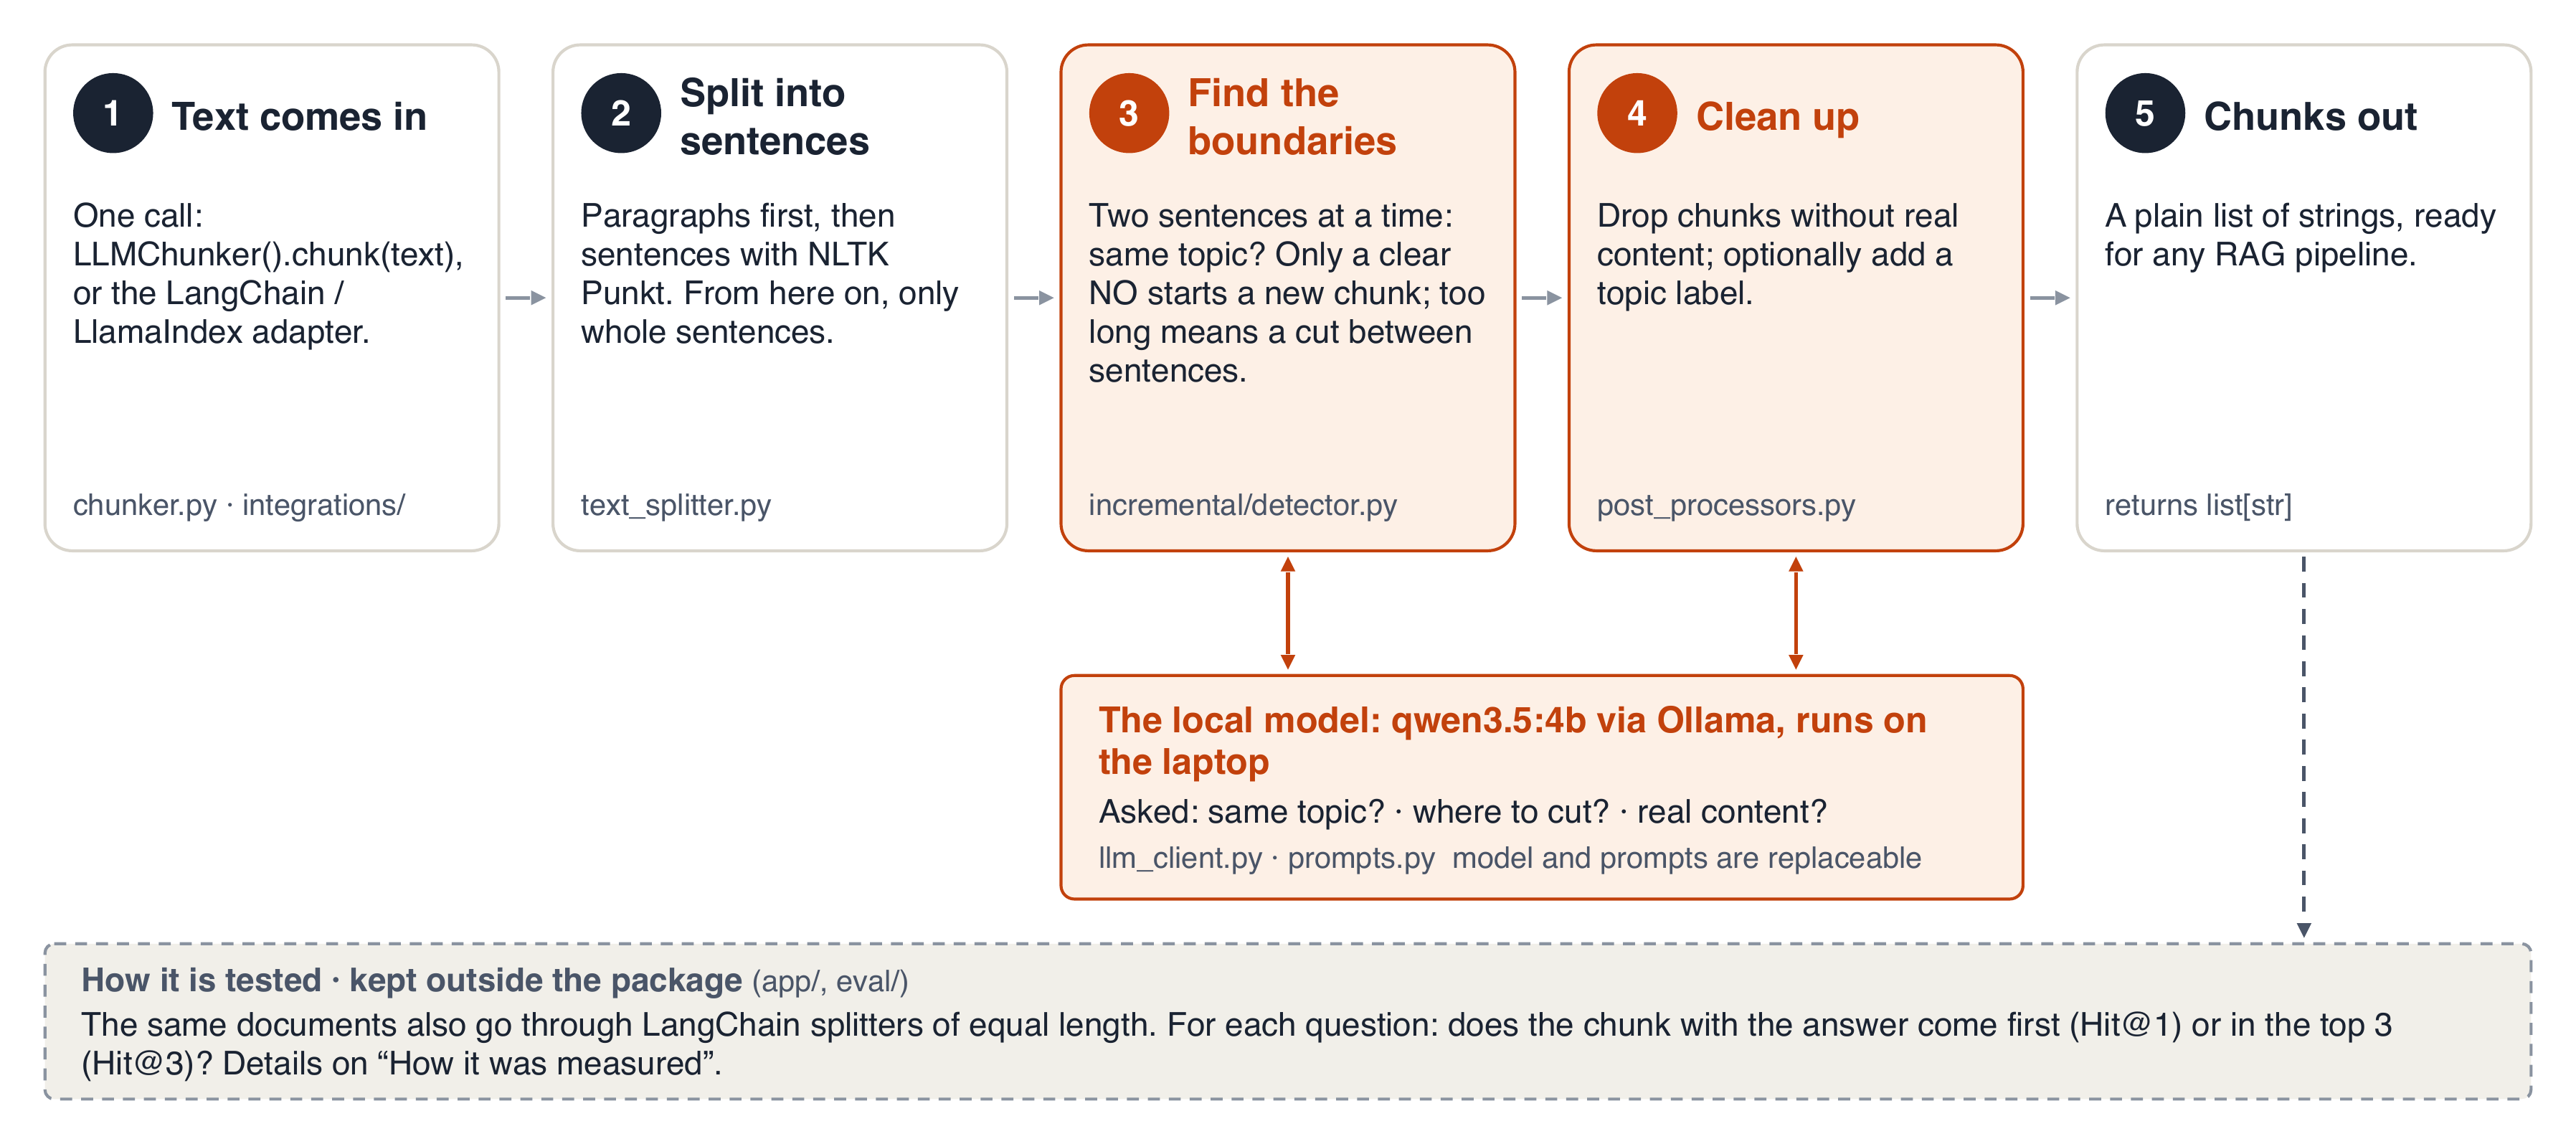
\includegraphics[width=\textwidth]{figures/architecture.png}
  \caption{Architecture of the library. A document passes five stages; the local
  model is asked during boundary detection (step 3) and by the optional
  post-processors (step 4). The evaluation harness is kept outside the package.}
  \label{fig:pipeline}
\end{figure}

\subsection{Boundary detection and size cap}
\label{sec:impl-incremental}
\label{sec:impl-sizecap}

The LLM-based chunking rests on two principles. First, the decision whether a sentence
belongs to the current chunk is \emph{incremental}: the model never sees the whole
document, only the current chunk and the next few sentences. This keeps every LLM call far
below the context window (4096 tokens by default) and makes the cost linear in the
document length. Second, merging is implicit: sentences are joined into chunks while the
model moves through the document, not in a separate step afterwards. \Cref{lst:loop} shows
the core of the loop.

\begin{lstlisting}[caption={The assembly loop, condensed.},label={lst:loop}]
while pos < len(sentences):
    candidate = sentences[pos:pos + self.step_sentences]
    pos += self.step_sentences

    if not current:                                  # first group of a chunk
        current = list(candidate)
    elif self._same_topic(current, candidate, pos):  # one LLM call
        current.extend(candidate)
    else:                                            # topic boundary
        chunks.append(" ".join(current))
        current = list(candidate)

    while self._over_limit(current):                 # size cap, see below
        idx = self._fit_split(current)
        chunks.append(" ".join(current[:idx]))
        current = current[idx:]
\end{lstlisting}

The condition for closing a chunk and starting a new one is deliberately conservative.
Only an explicit NO from the model sets a boundary; an unclear answer continues the
current chunk. The reason is that, because the process is incremental, a wrong split
cannot be repaired later, whereas a missed boundary merely produces a longer chunk.

The topic decisions alone put no upper limit on chunk length: a twenty-page document about
one subject would in theory become a single, unusable chunk. The settings
\code{max\_chunk\_sentences} and \code{max\_chunk\_chars} therefore force a split once a
chunk exceeds either threshold, regardless of the topic.

Two policies decide where this cut is made, and both cut only between sentences. With
\code{smart\_split}, the default, the model reads the over-long chunk and chooses the
sentence at which the split fits best; the chunker then moves this index backwards until
the first piece fits the character cap. With \code{smart\_split} disabled, the oversized
chunk is cut at its middle sentence. The two policies form one of the ablations in
\cref{sec:ablations}: they differ only in where the cap cuts, not in whether it applies.

The size cap is a target, not a guarantee. Because cuts are only made at sentence
boundaries, a single sentence that is longer than \code{max\_chunk\_chars} is never split
and becomes a chunk that exceeds the cap.

\subsection{Heading awareness and post-processing}
\label{sec:impl-headings}
\label{sec:impl-postproc}

In addition to the topic decisions, the library can force a boundary at headings, a
feature that was added during the evaluation. It implements three ways of finding
headings. The default mode \code{"regex"} applies a fixed pattern for numbered and named
headings to the sentences after tokenisation. Its successor, the mode \code{"lines"},
works on the raw text before tokenisation and catches headings such as \code{3.2. Error
Handling} that the sentence tokeniser would otherwise break apart. The mode
\code{"hybrid"} additionally asks the model about short sentence groups that the pattern
did not flag, which makes it possible to measure the model's contribution to heading
detection.

Two optional post-processing steps run over the finished chunk list: the low-information
filter and the topic enricher. A third one, a merging step, was considered during the
design but became unnecessary, because the incremental mode merges while it moves through
the document and never revisits chunks it has already closed. In the legacy mode
\code{"window"}, a separate merging step caused errors: the pre-split pieces could already
contain different topics, and a wrong merge diluted the chunk.

The \emph{low-information filter} asks the model for each chunk whether it contains
substantive information. Only an explicit NO removes the chunk; the aim is to keep bare
headings, boilerplate lines and similar fragments out of the index. Its effect depends
strongly on the document: manuals and table-heavy texts lose more chunks than continuous
prose such as a non-fiction book.

The \emph{topic enricher} prefixes each chunk with an LLM-generated line
\code{[Topic: \ldots]}, so that a chunk that is taken out of its document and loses its
context still carries a short descriptive label. Enrichment is disabled by default,
whereas the low-information filter is enabled. Their effects are evaluated in
\cref{sec:filter}.

\subsection{Configuration and the LLM client}
\label{sec:impl-client}

All chunker settings are collected in \code{ChunkerConfig}, an immutable dataclass that
validates itself on construction, so that an invalid setting fails before the chunking
starts. The chunker accepts either a configuration object or the individual settings as
keyword arguments, but refuses both at once, since it would be ambiguous which one takes
precedence. The client, \code{OllamaClient}, wraps Ollama's chat endpoint and adds three
mechanisms that make the output reproducible and complete.

\begin{description}
    \item[Deterministic decoding.] The temperature is set to zero and the seed is fixed
    (\code{temperature=0}, \code{seed=42}), so that repeated runs produce identical
    output (\cref{sec:verify-determinism}).

    \item[A prompt-size guard.] Ollama silently truncates a prompt that exceeds
    \code{num\_ctx}, so the model would judge a chunk of which it sees only a part. The
    client therefore estimates the size of each prompt before sending it (four characters
    per token) and refuses a prompt that would exceed \SI{90}{\percent} of
    \code{num\_ctx}, rather than letting a truncated judgement propagate through the
    chunking. A second check reads the token count that Ollama reports back and logs a
    warning when the prompt comes close to the limit.

    \item[Retries.] Server errors (5xx) and transport errors, such as a model reload or a
    dropped connection, are retried with exponential backoff, while client errors (4xx)
    are raised at once.
\end{description}

\section{Developer guide}
\label{sec:developer-guide}

This section is a guide for developers who want to use the library. It covers the
installation, the three ways of calling the chunker (the native API and two framework
adapters) and the extension points.

\subsection{Installation and native API}
\label{sec:install}
\label{sec:native-api}

The library is published on the Python Package Index as
\code{llm-semantic-chunker}\footnote{\url{https://pypi.org/project/llm-semantic-chunker/}}:

\begin{lstlisting}[language=bash,caption={Installing the library and its optional extras.},label={lst:install}]
pip install llm-semantic-chunker
pip install "llm-semantic-chunker[langchain]"     # LangChain adapter
pip install "llm-semantic-chunker[llamaindex]"    # LlamaIndex adapter, Python 3.10+
pip install "llm-semantic-chunker[pdf]"           # PDF text extraction
pip install "llm-semantic-chunker[vectorstore]"   # ChromaDB wrapper
\end{lstlisting}

The base installation brings only the three runtime dependencies named in
\cref{sec:impl-overview} and is sufficient to chunk strings; everything beyond that is an
extra that is installed on demand.

The chunker is meant to be a small component of a larger pipeline. Computing embeddings
in-process with sentence-transformers would have turned an installation of about
\SI{40}{\mega\byte} into one of well over \SI{800}{\mega\byte} and tied every project using
the library to the PyTorch version used here. Delegating the embeddings to a second
Ollama-served model avoids this dependency instead of hiding it behind an optional extra.
It also needs less memory, which was decisive given the hardware constraints described in
\cref{sec:impl-overview}.

Chunking also requires a local Ollama chat model. The default is \code{qwen3.5:4b}, but any
other Ollama model can be set in the client. On its first call, the sentence splitter
downloads NLTK's punkt data once; later runs reuse it.

Once installed, the chunker is called through its native API (\cref{lst:native}).

\begin{lstlisting}[caption={Chunking a string with the native API.},label={lst:native}]
from llm_semantic_chunker import LLMChunker, OllamaClient

chunker = LLMChunker(client=OllamaClient(), max_chunk_chars=1200)
chunks = chunker.chunk(text)          # -> list[str]
\end{lstlisting}

The return value is a plain list of strings. Character offsets, the governing heading and
similar metadata were deliberately left out, because this work is limited to evaluating
whether LLM-based chunking sets better boundaries than the baseline strategies.

\subsection{Framework adapters and extension points}
\label{sec:integrations}
\label{sec:extending}

The frameworks are integrated through adapters, so that an existing splitter can be
replaced without changing the rest of a pipeline (\cref{lst:adapters}).
\code{LLMSemanticSplitter} implements LangChain's \code{TextSplitter} interface, so that
the methods \code{create\_documents()}, \code{split\_documents()} and
\code{transform\_documents()} come from the base class. \code{LLMSemanticNodeParser} does the same for LlamaIndex: it
subclasses the \code{TextSplitter} of LlamaIndex, which is itself a \code{NodeParser}, so
that the method \code{get\_nodes\_from\_documents()} works directly. In both frameworks,
the adapter only implements \code{split\_text()}; everything else is built on top of it.

\begin{lstlisting}[caption={Replacing an existing splitter. Only the constructor
line changes.},label={lst:adapters}]
# instead of: RecursiveCharacterTextSplitter(chunk_size=700, chunk_overlap=50)
from llm_semantic_chunker.integrations.langchain import LLMSemanticSplitter
splitter = LLMSemanticSplitter(max_chunk_chars=1200)
docs = splitter.create_documents([text])        # -> list[Document]

# instead of: SentenceSplitter(chunk_size=700, chunk_overlap=50)
from llm_semantic_chunker.integrations.llamaindex import LLMSemanticNodeParser
parser = LLMSemanticNodeParser(max_chunk_chars=1200)
nodes = parser.get_nodes_from_documents([Document(text=text)])  # -> list[TextNode]
\end{lstlisting}

The LlamaIndex extra requires Python 3.10 or newer, because \code{llama-index-core}
depends on \code{banks}, which annotates fields as \code{Path | None}. This syntax raises a
\code{TypeError} on Python 3.9, which the chunker itself still supports. LlamaIndex is
therefore kept in a separate extra.

Beyond the adapters, the library has three extension points and one deliberate exception.

\paragraph{The language model.} Any object with a \code{chat(messages) -> str} method can
be passed as \code{client}, for example a wrapper around a hosted API or another local
server.

\paragraph{The prompts.} Each kind of model decision has its own prompt class, which can
be extended or replaced through a keyword argument: \code{incremental\_prompt} for judging
topic shifts, \code{low\_info\_prompt} for removing low-information chunks and
\code{enrichment\_prompt} for adding a topic line.

\paragraph{Logging.} All library messages go through the \code{logging} module behind a
\code{NullHandler}, so that the application decides what is shown; \code{verbose=True}
only attaches a console handler to the package logger.

\paragraph{What is not replaceable.} The assembly loop. It defines the LLM-based strategy
itself, and changing it would interfere with the structure of the project.

\section{Evaluation harness and verification}
\label{sec:harness}
\label{sec:testing}

The evaluation harness is configured by a \code{ChunkerConfig} and an \code{EvalConfig}.
\code{Pipeline} takes a document and runs two phases: first chunk and cache, then embed,
retrieve and score. \code{StrategyCollector} assembles the baseline strategies, the LLM
chunker and all ablation arms, each of which differs from the reference configuration in
exactly one setting. Two safeguards keep the cached chunks consistent. First, each arm's
cache name is derived from its configuration, so that a setting and its cached file cannot
drift apart. Second, each cache stores a fingerprint of the code that drew its boundaries,
a hash over the syntax trees of the relevant modules, so that results from different code
versions cannot be mixed.

Two further checks verify the determinism of the library and the validity of the question
sets. The scripts are in the repository under \code{eval/experiments/} and \code{tools/}.

\paragraph{Determinism.}
\label{sec:verify-determinism}
The evaluation relies on the chunking being deterministic. Repeating full chunking runs of
the evaluated documents would have taken days, so \code{run\_determinism.py} tests this on
a shorter document instead: it chunks the document several times with identical settings
and compares a hash over the chunk lists. In three runs, it produced \num{48} chunks each
with a mean length of \num{673} characters, the identical digest and identical boundary
statistics (\num{27} topic decisions, \num{28} size-cap splits, \num{8} heading and \num{9}
end boundaries, counted before the low-information filter).

\paragraph{Question sets.}
\label{sec:verify-questions}
\code{tools/verify\_questions.py} tests every question against its document. The anchor
must occur in the document verbatim after whitespace normalisation and exactly once, it
must be at least 40 characters long, and no anchor may appear twice in a set. All
\num{1483} anchors of the three sets used in \cref{ch:evaluation} pass, with lengths
between \num{60} and \num{297} characters.

\section{Availability and use of AI tools}
\label{sec:ai-usage}
\label{sec:availability}

The source code is available at \url{https://github.com/antunoviic/semantic-chunking}
under the MIT license, and the library is published on PyPI as \pkg{} (version 1.0.2).
Besides the library, the repository contains the evaluation harness, the three evaluated
documents, the question sets and the chunk lists of the evaluated arms, so that the
evaluation of \cref{ch:evaluation} can be repeated without chunking the documents again.

Claude Code, with different Claude models, was used in VS Code as a pair programmer for
the library and the evaluation harness. It wrote and ran most of the evaluation and
analysis scripts and reviewed code and results. It was also used for research for this
thesis, to build tables and figures, for the presentation, and to proofread the text of
this thesis for spelling, grammar and consistency. Furthermore, the question sets of
\cref{ch:evaluation} were generated by an external language model (Claude Sonnet 5) as
part of the method (\cref{sec:questions}). The research methods, the choice of documents
and the design, architecture and implementation decisions were not delegated to AI tools.
Every review finding was checked against the code or measured before it was accepted, and
the main results were recomputed by a second, independent implementation
(\cref{sec:robustness}).

\chapter{Evaluation}
\label{ch:evaluation}

This chapter evaluates whether the chunks produced by the library of
\cref{ch:implementation} are retrieved more accurately than those of the baseline
strategies. After the datasets (\cref{sec:datasets}) and the design (\cref{sec:design}),
\cref{sec:results} reports the main comparison;
\cref{sec:further} examines the source of the
differences, the low-information filter and the other configuration options and
parent-child retrieval, and \cref{sec:threats} discusses robustness and validity. \Cref{ch:lessons} interprets the results.

\section{Datasets and question sets}
\label{sec:datasets}

The evaluation uses three documents, one for each structure class of
\cref{sec:commitments} (\cref{tab:datasets}).

\begin{table}[htbp]
  \centering
  \caption{Evaluation documents. Characters after text extraction, sentences as counted by
  the library's sentence splitter, and questions that passed the verification
  (\cref{sec:questions}).}
  \label{tab:datasets}
  \small
  \begin{tabular}{@{}lL{5.4cm}lrrr@{}}
    \toprule
    Document & Source and format & Structure class & Characters & Sentences & Questions \\
    \midrule
    \code{rfc9110} & RFC 9110, HTTP Semantics~\cite{rfc9110}; plain text & explicit & \num{502906} & \num{3882} & 549 \\
    \code{nasa}    & NASA Systems Engineering Handbook~\cite{nasa2016handbook}; PDF, 297 pages & implicit & \num{813744} & \num{6071} & 534 \\
    \code{wells}   & H.\,G.~Wells, \emph{A Short History of the World}~\cite{wells1922history}; plain text & unstructured & \num{616390} & \num{4754} & 400 \\
    \bottomrule
  \end{tabular}
\end{table}

\code{rfc9110} is an explicit text: a technical standard with numbered sections
throughout. \code{wells} is continuous narrative prose about different historical periods,
in which the topic shifts are fluid throughout the document. \code{nasa} (NASA
SP-2016-6105 Rev2) changes topic from paragraph to paragraph, but loses its layout during
text extraction. The project's PDF reader joins the lines of a page into one paragraph
(310 paragraphs, median \num{2830} characters), and the running header appears inside the
text on almost every page.

\paragraph{Question sets.}
\label{sec:questions}
The questions were generated by an external language model (Claude Sonnet 5), never by the
local model under test. The prompt requires every question to come with an anchor: a
passage of 60 to 300 characters, copied verbatim from the document, that contains the
answer. Furthermore, the prompt requires a question to be answerable from one section
alone and its anchor to appear only once in the text. An automatic check
(\cref{sec:verify-questions}) then tests every candidate against the extracted text: the
anchor must be verbatim after normalisation, at least 40 characters long, not duplicated
and unique in the document. Candidates that fail are discarded (16 of 550 on \code{nasa},
4 of 553 on \code{rfc9110}). No questions were removed or added by hand afterwards.

\section{Experimental design}
\label{sec:design}

\subsection{Compared strategies}

The LLM chunker is evaluated in two arms that share one configuration: two sentences per
decision (\code{step\_sentences=2}), a size cap of \num{1200} characters, at most 100
sentences per chunk and no heading detection. The \emph{tested arm} also switches off the
low-information filter, which the library enables by default, so that it evaluates the
chunking alone, without any post-processing. The \emph{filter arm} is the same
configuration with the filter; it shows the effect of the filter as an optional add-on
(\cref{sec:filter}) and is the reference for the ablations (\cref{sec:ablations}).
\Cref{tab:strategies} lists the five baselines.

\begin{table}[htbp]
  \centering
  \caption{Baselines. All are length-matched to the LLM chunker (see text).}
  \label{tab:strategies}
  \small
  \begin{tabular}{@{}L{3.2cm}L{11.3cm}@{}}
    \toprule
    Strategy & Implementation \\
    \midrule
    Fixed-size & LangChain \code{CharacterTextSplitter}, space as separator, overlap of 50 characters. \\
    Recursive (default) & LangChain \code{RecursiveCharacterTextSplitter} with its default separator order: paragraph, line break, space. A paragraph longer than the target is cut at the last space that fits, usually inside a sentence. Overlap of 50 characters. \\
    Recursive (sentence ends) & The same class with a sentence end (whitespace after \code{.}, \code{!} or \code{?}) as second separator, before line break and space, so that an over-long paragraph is cut after the last complete sentence that fits. Overlap of 50 characters. \\
    Semantic (tuned) & LangChain \code{SemanticChunker} with the same bge-m3 embeddings. The percentile threshold is set by bisection to reach the target length, and chunks above \num{1200} characters are divided at sentence boundaries. \\
    Packing (no model) & The library's own \code{LLMChunker} with a stand-in client that always answers \enquote{same topic}, so that every boundary comes from the size cap, which cuts between sentences (at the middle sentence). \\
    \bottomrule
  \end{tabular}
\end{table}

\paragraph{Length matching.} Because chunk length can influence the hit rates, every
baseline is tuned to the mean length of the LLM chunks that the filter keeps (714
characters on \code{nasa}, 720 on \code{rfc9110}, 725 on \code{wells}). The tested arm's
own mean is lower (454, 621 and 711 characters), because it also contains the chunks that
the filter removes, mostly short fragments such as 464 chunks of the \code{nasa} table of
contents that consist of nothing but dot leaders. A splitter's mean length cannot be set
directly, so its parameters (chunk size, percentile threshold etc.) are adjusted until the
mean lies within \SI{4}{\percent} of the target.

\subsection{Retrieval, hit criterion and statistical analysis}
\label{sec:stats}

Chunks and questions are embedded with bge-m3~\cite{chen2024bgem3}, served by a local
Ollama instance. Retrieval uses exact search: each question is compared with every chunk
by cosine similarity, and the chunks are ranked by this score. The approximate HNSW
index~\cite{malkov2020hnsw} that the project's vector store uses by default does not
guarantee the true nearest neighbours; in this project, its ranking changed each time the
same data was indexed again, so it was not used for the final results.

Each question is judged by how much of its anchor is present in a chunk. A question counts
as a hit at rank $k$ (\hitk{k}) if one of the $k$ highest-ranked chunks contains at least
\SI{80}{\percent} of the anchor as one continuous passage. The threshold accepts an anchor
whose last words fall into the next chunk, but not one that a chunk boundary splits in
half. Line breaks and repeated spaces are ignored, so that formatting differences between
document and chunks do not matter, and the passage must be continuous, so that a chunk
does not count merely because it shares words with the anchor. Applied to all chunks of a
strategy instead of only the top $k$, the same test gives the share of \emph{anchors
intact}: if no chunk contains at least \SI{80}{\percent} of the anchor, the chunking has
cut the answer apart and no retriever can find it. This share is therefore an upper bound
for \hitk{k} at every $k$. \hitk{1} and \hitk{3} are the reported metrics.

A potential downside of this approach is that the hit criterion favours large chunks: the larger a chunk, the more likely it is to
contain a given anchor, and with one chunk per document every question would be a hit at
$k=1$. However, two measures prevent this effect from deciding the comparison. First, all
baselines are length-matched to the LLM chunker (\cref{sec:design}), so that no strategy
has larger chunks on average and the remaining differences stem from where the boundaries
are placed, not from how large the chunks are. Second, the LLM chunker and the tuned
semantic chunker are limited by a size cap of \num{1200} characters, so that no chunk can
span large parts of a document. In practice, such chunks would also be of little use,
since they dilute the embedding and fill the context of the generating model with
irrelevant text (\cref{sec:rag_chunking}), which would lead to worse answer generation.

\paragraph{Statistical analysis.} All strategies are evaluated on the same questions, so they
can be compared question by question. When the tested arm is compared with one baseline, only the questions on which
the two disagree are informative: $b$ is the number of questions that only the LLM arm
answers, and $c$ the number that only the baseline answers. Questions that both or neither
answer are ignored. If both strategies were equally good, each of these disagreements
would go to the LLM arm or to the baseline with a probability of $1/2$. The exact McNemar
test~\cite{mcnemar1947} computes the two-sided probability $p$ of a split at least as
uneven as the observed one under this assumption. The size of the effect is the
difference in hit rate, $d = (b-c)/n$ with $n$ questions, in percentage points (pp), with a
\SI{95}{\percent} Wald interval for paired proportions,
$d \pm 1.96\sqrt{\bigl((b+c)/n - d^2\bigr)/n}$, which gives the range of differences
compatible with the data; an interval that contains zero means that no difference can be
established. The intervals are not adjusted for multiple testing.

The tested arm is compared with five baselines on three documents at two values of $k$,
which gives a total of 30 tests. Holm's procedure~\cite{holm1979} controls the family-wise
error rate, the probability of at least one false positive among the 30 tests, at
$\alpha = 0.05$: the $p$-values are sorted in ascending order, the $i$-th smallest is
compared with $\alpha/(30-i+1)$, and the procedure stops at the first comparison that
fails. Equivalently, the $i$-th smallest $p$-value is multiplied by $30-i+1$, capped at 1
and never allowed to fall below the adjusted value before it; these \emph{adjusted}
$p$-values are reported and can be compared with $\alpha$ directly, whereas
\emph{unadjusted} values refer to a single test.

\section{Results}
\label{sec:results}

\begin{table}[htbp]
  \centering
  \caption{Hit rates in percent. The tested arm is compared with the five baselines;
  the filter arm with the low-information filter as an add-on is shown for reference
  (\cref{sec:filter}).}
  \label{tab:results}
  \small
  \begin{tabular}{@{}lrrrrrr@{}}
    \toprule
    & \multicolumn{2}{c}{\code{nasa} ($n=534$)} & \multicolumn{2}{c}{\code{rfc9110} ($n=549$)} & \multicolumn{2}{c}{\code{wells} ($n=400$)} \\
    \cmidrule(lr){2-3}\cmidrule(lr){4-5}\cmidrule(l){6-7}
    Strategy & \hitk{1} & \hitk{3} & \hitk{1} & \hitk{3} & \hitk{1} & \hitk{3} \\
    \midrule
    LLM (tested arm) & 69.5 & 87.1 & 74.9 & 90.2 & 84.0 & 92.8 \\
    Recursive (sentence ends) & 66.9 & 84.3 & 71.6 & 88.0 & 89.8 & 96.2 \\
    Packing (no model) & 64.8 & 82.6 & 71.6 & 87.4 & 86.5 & 94.8 \\
    Semantic (tuned) & 66.5 & 83.3 & 73.6 & 89.8 & 83.2 & 93.8 \\
    Recursive (default) & 61.6 & 80.3 & 71.8 & 88.0 & 87.2 & 95.0 \\
    Fixed-size & 61.2 & 76.8 & 58.5 & 80.5 & 77.8 & 89.8 \\
    \addlinespace
    LLM with filter (add-on) & 68.0 & 83.5 & 73.6 & 88.3 & 84.0 & 92.8 \\
    \bottomrule
  \end{tabular}
\end{table}

\Cref{tab:results} shows a pattern that the individual tests confirm. On \code{nasa} and
\code{rfc9110}, the tested arm reaches the highest hit rates of the six compared
strategies at both $k$ (\hitk{1} \SI{69.5}{\percent} and \SI{74.9}{\percent}), but it
leads the sentence-aware baselines by only 0.4 to 4.7~pp. On \code{wells}, three baselines
are ahead of it; the clear winner, the recursive splitter with sentence ends, reaches
\SI{89.8}{\percent} against \SI{84.0}{\percent}. Fixed-size splitting is the weakest
strategy on every document. At $k=3$, most differences on \code{rfc9110} and \code{wells}
shrink, because a passage missed at rank~1 is often found at rank~2 or~3.

\begin{figure}[htbp]
  \centering
  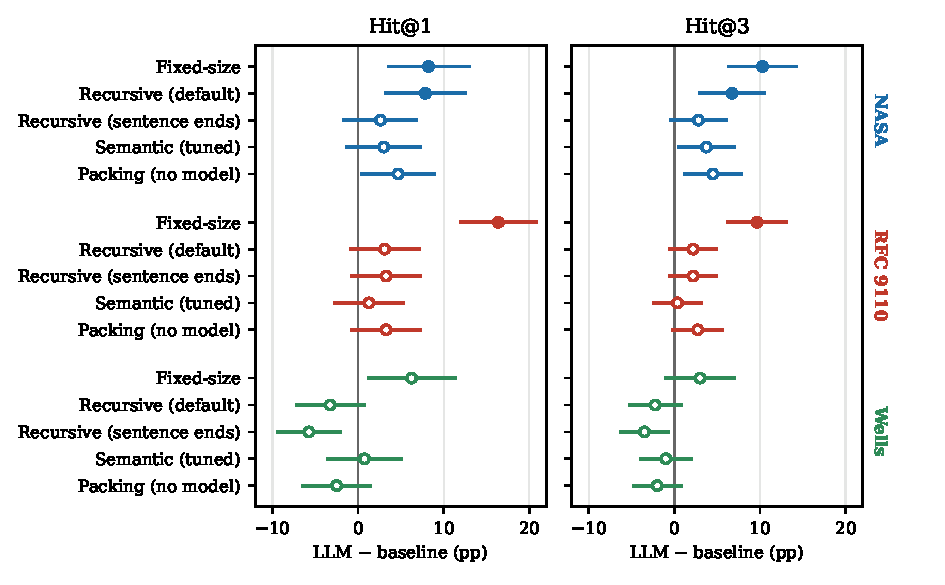
\includegraphics[width=\textwidth]{figures/forest_v4.pdf}
  \caption{Difference in hit rate between the tested LLM arm and each baseline, with
  \SI{95}{\percent} intervals. Filled markers are significant after the Holm correction
  over all 30 tests. Values right of zero favour the LLM chunker.}
  \label{fig:forest}
\end{figure}

Six of the 30 comparisons remain significant after the Holm correction, all against the
two naive splitters. Against fixed-size splitting, the tested arm leads on \code{rfc9110}
by $+16.4$~pp at \hitk{1} [$+12.0$, $+20.8$] and $+9.7$~pp at \hitk{3} [$+6.2$, $+13.1$],
and on \code{nasa} by $+8.2$ and $+10.3$~pp (adjusted $p \le 0.021$). Against LangChain's
default recursive splitter, it leads on \code{nasa} by $+7.9$~pp at \hitk{1} [$+3.2$,
$+12.5$] and $+6.7$~pp at \hitk{3} (adjusted $p = 0.030$ and $0.014$). The nearest miss is
in the opposite direction: the lead of the recursive splitter with sentence ends on
\code{wells} ($-5.8$~pp at \hitk{1}), which is not significant after the Holm correction
(adjusted $p = 0.064$).

\Cref{fig:forest} makes the structure of the result visible. Against fixed-size splitting,
all four intervals on \code{nasa} and \code{rfc9110} lie above zero; against the default
recursive splitter, the two on \code{nasa} do. Against the three baselines that keep
sentences intact (recursive with sentence ends, the tuned semantic chunker and packing
without the model), the point estimates on \code{nasa} and \code{rfc9110} lie between
$+0.4$ and $+4.7$~pp, and nine of the twelve intervals contain zero. On \code{wells}, the
LLM arm is behind three of the five baselines at \hitk{1} and four at \hitk{3}.

\section{Further analyses}
\label{sec:further}

\subsection*{Where the differences come from}
\label{sec:mechanism}

\begin{table}[htbp]
  \centering
  \caption{Chunks ending inside a sentence (mid-sent.) and anchors contained to at least
  \SI{80}{\percent} in some chunk (intact), in percent.}
  \label{tab:mechanism}
  \small
  \begin{tabular}{@{}lrrrrrr@{}}
    \toprule
    & \multicolumn{2}{c}{\code{nasa}} & \multicolumn{2}{c}{\code{rfc9110}} & \multicolumn{2}{c}{\code{wells}} \\
    \cmidrule(lr){2-3}\cmidrule(lr){4-5}\cmidrule(l){6-7}
    Strategy & mid-sent. & intact & mid-sent. & intact & mid-sent. & intact \\
    \midrule
    LLM (tested arm) & 3.1 & 98.7 & 11.9 & 99.3 & 7.1 & 95.0 \\
    Recursive (sentence ends) & 19.3 & 98.9 & 35.2 & 99.6 & 16.0 & 99.5 \\
    Packing (no model) & 3.8 & 98.1 & 18.3 & 98.9 & 3.4 & 96.2 \\
    Semantic (tuned) & 3.4 & 97.9 & 6.5 & 98.9 & 1.2 & 95.8 \\
    Recursive (default) & 83.7 & 94.6 & 37.6 & 99.5 & 34.6 & 98.0 \\
    Fixed-size & 94.8 & 92.1 & 93.0 & 93.1 & 96.7 & 93.8 \\
    \addlinespace
    LLM with filter (add-on) & 4.0 & 93.6 & 9.2 & 97.3 & 6.0 & 95.0 \\
    \bottomrule
  \end{tabular}
\end{table}

The anchors are one or two sentences long, so a chunking that never cuts inside a sentence
keeps almost every anchor intact, whatever it does between sentences. \Cref{tab:mechanism}
shows the proportion of chunks that end without sentence-final punctuation, a proxy for a
cut inside a sentence. Fixed-size splitting ends 93 to \SI{97}{\percent} of its chunks
inside a sentence and leaves only 92 to \SI{94}{\percent} of the anchors intact.
LangChain's default recursive splitter performs better on \code{rfc9110} and \code{wells},
whose paragraphs are short, but on \code{nasa} it finds no paragraph break within the
target length and falls back to the space character, so that \SI{83.7}{\percent} of its
chunks end inside a sentence. This is where the LLM arm is furthest ahead, although the
situation is created primarily by the text extraction rather than by the document.

The strongest evidence on the contribution of the model comes from packing, which uses the
same sentence splitter and assembly loop without asking the model anything. It trails the
tested arm by 4.7~pp on \code{nasa} and 3.3~pp on \code{rfc9110} at \hitk{1}, neither
difference significant after the correction, and leads it by 2.5~pp on \code{wells}. On
\code{wells}, \SI{77}{\percent} of the LLM arm's boundaries are forced by the size cap
rather than set by a topic decision (on \code{nasa} \SI{46}{\percent}, on \code{rfc9110}
\SI{53}{\percent}), so there the chunker behaves largely like packing with a different
split point. The model's topic decisions produce boundaries that differ from packing, but
no retrieval benefit that remains significant after the correction.

\subsection*{The low-information filter and other options}
\label{sec:filter}

This section evaluates the optional features of the library: the low-information filter
as an add-on to the tested arm, and three further options as single-setting ablations.

\paragraph{Low-information filter.} The filter is an optional post-processing step: after
chunking, the model judges every chunk, and the ones without substantive information are removed. Added to the tested
configuration, it drops 761 of \num{1786} chunks on \code{nasa} but only
\SI{9.8}{\percent} of the text, mostly fragments such as the dot leaders of the table of
contents. It also deletes answers: 27 anchors of \code{nasa} and 11 of \code{rfc9110} are
no longer contained in any chunk. On \code{nasa}, 18 of these 27 lie in the reference
lists, from which the generating model produced 35 questions although the prompt excluded
them. As a result, the filter lowers \hitk{3} by 3.6~pp on \code{nasa} and by 1.8~pp on
\code{rfc9110} (Holm-adjusted $p = 0.002$ and $0.032$ over the six tests of this
comparison) and leaves \code{wells} unchanged.

The filter arm, tested against the five baselines with its own Holm family of 30 tests,
keeps only two significant results, both against fixed-size splitting on \code{rfc9110}
($+15.1$ and $+7.8$~pp). Its leads over the naive splitters on \code{nasa} at \hitk{1}
($+6.4$~pp against the default recursive splitter, $+6.7$~pp against fixed-size splitting)
are no longer significant (adjusted $p = 0.28$ and $0.18$), mainly because the filter
deletes passages that some questions ask about.

\label{sec:ablations}
Three further options of \cref{ch:implementation} were evaluated as single-setting changes
of the filter arm, the tested arm of the original design, produced in the same chunking run and
scored on the same questions. These comparisons are exploratory only; none of the
differences would survive a correction for multiple testing (the smallest unadjusted $p$
is 0.029).

\paragraph{Split point at the size cap.} Splitting an over-long chunk at its middle
sentence instead of at the point chosen by the model (\code{nasa} only) changes \hitk{1}
by $-0.2$~pp and \hitk{3} by $-2.2$~pp ($p = 0.13$).

\paragraph{Heading detection.} Neither heading mode (line pattern or hybrid with the
model) changes a hit rate by more than 0.7~pp on any document. On \code{wells}, the
line-pattern arm is identical to the reference, and on \code{nasa}, whose line structure
is lost in extraction, the chunk lists differ from the reference by only 7 (line pattern)
and 52 (with the model) chunks, so that heading detection has little to change on these
two documents.

\paragraph{Topic enrichment.} A model-generated topic line in front of each chunk lowers
\hitk{1} on all three documents ($-0.9$, $-2.2$ and $-1.8$~pp) and \hitk{3} as well. The
label therefore does not help the retriever find the passage.

\subsection*{Parent-child retrieval}
\label{sec:parentchild}

The evaluation harness also implements parent-child retrieval, a retrieval technique that
is independent of the chunking and is used here as an additional condition under which the
strategies are compared. Every chunk (the parent) is divided into children of 250
characters (with LangChain's recursive splitter and an overlap of 30 characters), the
children are embedded and searched, and the parents of the best children are returned,
each parent at most once. It was applied to the tested arm and to all five baselines, with
the same questions, search and hit criterion as in \cref{sec:results}.

\begin{table}[htbp]
  \centering
  \caption{Hit rates in percent with parent-child retrieval, applied to every strategy.
  In parentheses: change of \hitk{1} against the same strategy without parent-child
  (\cref{tab:results}), in pp.}
  \label{tab:parentchild}
  \small
  \begin{tabular}{@{}lrrrrrr@{}}
    \toprule
    & \multicolumn{2}{c}{\code{nasa}} & \multicolumn{2}{c}{\code{rfc9110}} & \multicolumn{2}{c}{\code{wells}} \\
    \cmidrule(lr){2-3}\cmidrule(lr){4-5}\cmidrule(l){6-7}
    Strategy & \hitk{1} & \hitk{3} & \hitk{1} & \hitk{3} & \hitk{1} & \hitk{3} \\
    \midrule
    LLM (tested arm) & 72.5 ($+3.0$) & 88.4 & 80.0 ($+5.1$) & 91.1 & 86.2 ($+2.2$) & 92.5 \\
    Recursive (sentence ends) & 73.0 ($+6.2$) & 87.6 & 82.9 ($+11.3$) & 92.7 & 90.0 ($+0.2$) & 97.5 \\
    Packing (no model) & 73.0 ($+8.2$) & 86.0 & 76.3 ($+4.7$) & 91.6 & 85.5 ($-1.0$) & 93.2 \\
    Semantic (tuned) & 71.2 ($+4.7$) & 88.2 & 77.6 ($+4.0$) & 90.5 & 89.0 ($+5.8$) & 94.5 \\
    Recursive (default) & 64.2 ($+2.6$) & 81.1 & 82.7 ($+10.9$) & 92.5 & 89.2 ($+2.0$) & 96.2 \\
    Fixed-size & 57.9 ($-3.4$) & 73.6 & 71.8 ($+13.3$) & 83.6 & 78.8 ($+1.0$) & 89.8 \\
    \bottomrule
  \end{tabular}
\end{table}

Parent-child raises most hit rates, but not evenly (\cref{tab:parentchild}), and the
baseline splitters gain the most on average. On \code{rfc9110}, the rule-based splitters
gain the most at \hitk{1} (fixed-size $+13.3$~pp, the two recursive splitters $+10.9$ and
$+11.3$~pp, against $+5.1$~pp for the LLM arm). On \code{nasa}, packing and the splitter
with sentence ends gain $+8.2$ and $+6.2$~pp against $+3.0$~pp for the LLM arm. On
\code{wells}, the changes are small except for the semantic chunker ($+5.8$~pp).

With parent-child applied to every strategy, the balance against the sentence-aware
baselines shifts towards the baselines. The recursive splitter with sentence ends combined
with parent-child retrieval reaches a higher \hitk{1} than the LLM chunker with or without
it on all three documents (\SI{73.0}{\percent}, \SI{82.9}{\percent} and
\SI{90.0}{\percent}), at no cost in model calls. Tested in the same way as in
\cref{sec:results}, with parent-child on both sides, the LLM arm remains significantly
ahead only of the two naive splitters (four tests on \code{nasa}, two on \code{rfc9110})
and is significantly behind the recursive splitter with sentence ends on \code{wells} at
\hitk{3} ($-5.0$~pp, adjusted $p = 0.040$).

\section{Robustness and threats to validity}
\label{sec:threats}

\label{sec:robustness}
The hit rates of all arms in \cref{tab:results} and the 30 tests of the filter arm were
recomputed by a second, independent implementation of the search, the hit criterion and
the tests, with identical results. \Cref{tab:sensitivity} shows how the result depends on
analysis decisions. The absence of a significant lead over the sentence-aware baselines
holds in every variant, and so does the lead over fixed-size splitting on \code{rfc9110}.
The lead over the naive splitters on \code{nasa} is less stable: it disappears when the
filter is added, and without the 35 questions from the reference lists, an exclusion
decided after seeing the results and therefore reported only as a sensitivity analysis,
the lead over the default recursive splitter at \hitk{1} is no longer significant,
although the one at \hitk{3} is.

\begin{table}[htbp]
  \centering
  \caption{Dependence of the result on analysis decisions. The \code{nasa} columns give
  the difference at \hitk{1} in pp with the Holm-adjusted $p$ in parentheses; the last
  column counts significant leads of the LLM arm over a sentence-aware baseline.}
  \label{tab:sensitivity}
  \small
  \begin{tabular}{@{}L{5.0cm}crrc@{}}
    \toprule
    & & \multicolumn{2}{c}{\code{nasa}, \hitk{1}} & \\
    \cmidrule(lr){3-4}
    Variant & Significant & vs.\ recursive & vs.\ fixed-size & Sentence-aware \\
    \midrule
    Main analysis (tested arm) & 6 of 30 & $+7.9$ (\textbf{0.030}) & $+8.2$ (\textbf{0.021}) & none \\
    Tested arm without the 35 reference-list questions (post hoc) & 5 of 30 & $+7.4$ (0.067) & $+8.0$ (\textbf{0.038}) & none \\
    Filter arm (original design) & 2 of 30 & $+6.4$ (0.279) & $+6.7$ (0.176) & none \\
    Filter arm without the 35 reference-list questions (post hoc) & 6 of 30 & $+8.2$ (\textbf{0.024}) & $+8.8$ (\textbf{0.012}) & none \\
    \bottomrule
  \end{tabular}
\end{table}

\paragraph{Internal validity.} The questions were generated by a language model, and 35 of
the \code{nasa} questions violate the generation rules, but they were kept because the
procedure fixed in advance allowed no manual removal. Exact search, the length target, the
additional baselines and the size of the test family were decided after the first test
runs were known (\cref{sec:lessons}), with the intention of making the comparison fairer.
The choice of the filter-free configuration as tested arm was made after the final results
were known and raises the number of significant tests from two to six, but both results
(with and without the filter) are reported. In addition, the fixed-size and default
recursive splitters use an overlap of 50 characters, whereas the other strategies use
none. The tested and the filter arm were chunked in two separate runs.

\paragraph{External validity.} Each structure class is represented by one document, so
class and document cannot be separated. \code{nasa} is the only PDF, and its extraction
favours every sentence-aware strategy there. One chunking model, one embedding model and
one parameter setting were evaluated.

\paragraph{Evaluation validity.} \hitk{$k$} on verbatim anchors measures whether the
passage containing the answer is retrieved intact, not whether an LLM answers correctly
based on the retrieved chunk or whether a chunk reads coherently. A chunking strategy that
keeps topics together but splits an anchor passage can therefore be penalised.

\chapter{Findings and Lessons Learned}
\label{ch:lessons}

\section{Summary of findings}
\label{sec:findings}

The research question asked whether a local language model places better chunk boundaries
than rule-based chunking techniques, and under which conditions. The evaluation of
\cref{ch:evaluation} answers it.

\paragraph{Better than splitters that cut sentences apart.} The LLM chunker retrieves
significantly better than fixed-size splitting and LangChain's default recursive splitter:
on \code{rfc9110} by $+16.4$~pp at \hitk{1} against fixed-size splitting, and on
\code{nasa} by $+8.2$ and $+7.9$~pp against the two. These gains mainly stem from the fact
that both baselines cut inside sentences. On \code{wells}, whose short paragraphs the
default recursive splitter keeps whole, no difference is significant.

\paragraph{Not better than splitters that keep sentences intact.} Against the recursive
splitter with sentence ends, the tuned semantic chunker and the same chunker without the
model, no significant difference remains. The LLM chunker leads by 0.4 to 4.7~pp on
\code{nasa} and \code{rfc9110} and is behind in five of six comparisons on \code{wells},
by up to 5.8~pp. None of these differences is significant, which indicates that once a
baseline keeps sentences intact, the decisions of the local model bring no measurable
gain.

\paragraph{The optional features do not improve retrieval.} The low-information filter
lowers \hitk{3} by 3.6~pp on \code{nasa} and 1.8~pp on \code{rfc9110} (\cref{sec:filter}).
Heading detection changes no hit rate by more than 0.7~pp, topic labels lower \hitk{1} on
all three documents, and letting the model choose the split point at the size cap makes no
significant difference (\cref{sec:ablations}). Parent-child retrieval raises most hit
rates, but the rule-based splitters gain more from it than the LLM chunker
(\cref{sec:parentchild}).

\paragraph{Cost and conclusion.} Although run times depend strongly on the hardware, LLM
chunking takes orders of magnitude longer than rule-based splitting: hours instead of about
a second per document. For retrieval as measured here, a length-matched recursive splitter
that prefers sentence ends to spaces reaches comparable hit rates, and combined with
parent-child retrieval it reaches a higher \hitk{1} than the LLM chunker on all three
documents. The cost of LLM-based chunking is paid only once, at indexing time, since
afterwards the chunks only have to be retrieved from the vector store. On the benchmarks
performed here, however, the difference in retrieval was not large enough to justify that
overhead.

\section{Lessons learned}
\label{sec:lessons}

The most challenging part of the project was the fair evaluation: building baselines that
are really comparable, measuring significance and separating the contribution of the
language model from that of the sentence splitting. The following lessons come from that
part.

\subsection{A fair comparison needs more than equal chunk length}

At first, only the mean chunk length of the baselines was adjusted to the LLM chunker.
Evaluating the first results revealed gaps in the experimental design: LangChain's
semantic chunker had to be tuned before it was a fair opponent, the recursive splitter
needed a variant that prefers sentence ends, and the same chunker without the model had to
be added to isolate the contribution of the model.

\subsection{Changes to the plan will happen}

The test configuration changed over time. For example, exact search replaced the
approximate index, and more baselines and a family of 30 tests were added after an
external review. Furthermore, the low-information filter was removed from the tested arm
because it removed passages that contained answers.

\subsection{Cached results ensure clean tracking}

Chunking takes hours, so the chunks have to be cached, and each cache needs a clear
fingerprint of its configuration and code, so that results from different states are not
mixed up.

\subsection{Working with limited hardware}

All runs used a laptop with \SI{8}{\giga\byte} of memory, and chunking one document took
two to six hours. Computing the embeddings in Ollama instead of the Python process and
caching every arm separately made the runs possible. The run time is one of the reasons
why the evaluation covers only three documents.

\section{Limitations and future work}
\label{sec:future}

The evaluation covers one document per structure class, the chunking model is a local
model with four billion parameters, and the embedding model and the parameter settings
were fixed for the entire project. Furthermore, the benchmark measures whether a verbatim
passage is retrieved intact, with questions generated by a language model; it does not
measure the quality of generated answers or whether a chunk reads as one coherent unit.
The results on \code{nasa} depend on an extraction that joins each page into one
paragraph, and the ablations were run only with the low-information filter.

Future work can address these limitations with several documents per structure class, a
larger chunking model, an end-to-end evaluation of the generated answers, a repetition on
\code{nasa} with a layout-preserving extraction and ablations without the filter. For the
library, returning the offsets of each chunk and the reason for each boundary (topic
decision, size cap or heading) instead of plain strings would make its decisions easier to
inspect in an application.


\printbibliography[heading=bibintoc,title={Bibliography}]

\end{document}
